%%%%%%%%%%%%%%%%%%%%%%%%% NOTE %%%%%%%%%%%%%%%%%%%%%%%%%%%%
%% You can ignore everything from here until             %%
%% "Question 1: Introduction"                            %%
%%%%%%%%%%%%%%%%%%%%%%%%%%%%%%%%%%%%%%%%%%%%%%%%%%%%%%%%%%%
\documentclass[8pt]{article}
\usepackage{amsmath, amsfonts, amsthm, amssymb}  % Some math symbols
\usepackage{fullpage}
\usepackage{graphicx}
\usepackage[x11names, rgb]{xcolor}
\usepackage{graphicx}
\usepackage{tikz}
\usepackage{tcolorbox}
\usetikzlibrary{decorations,arrows,shapes}
\usepackage{float} % Add this package to control float placement
\usepackage{etoolbox}
\usepackage{enumerate}
\usepackage{listings}
\lstset{
    language=Python,           % Set the language of the code
    basicstyle=\footnotesize\ttfamily,
    keywordstyle=\color{blue}, % Set color for keywords
    commentstyle=\color{gray}, % Set color for comments
    stringstyle=\color{red},   % Set color for strings
    numbers=left,              % Display line numbers on the left
    numberstyle=\tiny\color{gray}, % Style for line numbers
    frame=single,              % Add a frame around the code
    breaklines=true            % Allow line breaking
}


\setlength{\parindent}{0pt}
\setlength{\parskip}{5pt plus 1pt}

\newcommand{\N}{\mathbb N}
\newcommand{\E}{\mathbb E}
\newcommand{\V}{Var}
\renewcommand{\P}{\mathbb P}
\newcommand{\f}{\frac}


\newcommand{\nopagenumbers}{
    \pagestyle{empty}
}

\def\indented#1{\list{}{}\item[]}
\let\indented=\endlist

\providetoggle{questionnumbers}
\settoggle{questionnumbers}{true}
\newcommand{\noquestionnumbers}{
    \settoggle{questionnumbers}{false}
}

\newcounter{questionCounter}
\newenvironment{question}[2][\arabic{questionCounter}]{%
    \addtocounter{questionCounter}{1}%
    \setcounter{partCounter}{0}%
    \vspace{.25in} \hrule \vspace{0.4em}%
        \noindent{\bf \iftoggle{questionnumbers}{#1: }{}#2}%
    \vspace{0.8em} \hrule \vspace{.10in}%
}{$ $\newpage}

\newcounter{partCounter}[questionCounter]
\renewenvironment{part}[1][\alph{partCounter}]{%
    \addtocounter{partCounter}{1}%
    \vspace{.10in}%
    \begin{indented}%
       {\bf (#1)} %
}{\end{indented}}

\def\show#1{\ifdefempty{#1}{}{#1\\}}

\newcommand{\header}{%
\begin{center}
    {\Large \show\myhwname}
    \show\myname
    \show\myemail
    \show\mysection
    \show\hwname
\end{center}}

\usepackage{hyperref} % for hyperlinks
\hypersetup{
    colorlinks=true,
    linkcolor=blue,
    filecolor=magenta,      
    urlcolor=blue,
}

%%%%%%%%%%%%%%%%% Identifying Information %%%%%%%%%%%%%%%%%
%% For 312, we'd rather you DIDN'T tell us who you are   %%
%% in your homework so that we're not biased when        %%
%% So, even if you fill this information in, it will not %%
%% show up in the document unless you uncomment \header  %%
%% below                                                 %%
%%%%%%%%%%%%%%%%%%%%%%%%%%%%%%%%%%%%%%%%%%%%%%%%%%%%%%%%%%%
\newcommand{\myhwname}{DS288 (AUG) 3:0 Numerical Methods }
\newcommand{\myname}{Naman Pesricha }
\newcommand{\myemail}{namanp@iisc.ac.in}
\newcommand{\hwname}{\textbf{Homework-5}}
\newcommand{\mysection}{SR - 24115}
%%%%%%%%%%%%%%%%%%%%%%%%%%%%%%%%%%%%%%%%%%%%%%%%%%%%%%%%%%%

%%%%%%%%%%%%%%%%%%% Document Options %%%%%%%%%%%%%%%%%%%%%%
\noquestionnumbers
\nopagenumbers
%%%%%%%%%%%%%%%%%%%%%%%%%%%%%%%%%%%%%%%%%%%%%%%%%%%%%%%%%%%

\begin{document}
\header

\begin{question}{Q1 Derive Simpsons Rule with error term by using

 $$\int_{x_0}^{x_2} f(x) \, dx = a_0 f(x_0) + a_1 f(x_1) + a_2 f(x_2) + k f^{(4)}(\xi)$$
 Find $a_0$, $a_1$, and $a_2$ from the fact that Simpson's rule is exact for $f(x) = x^n$ when
 n = 0, 1, 2, and 3. Then find $k$ by applying the integration formula to f(x) = $x^4$. [3
    points]
}
We use equispaced points for Simpson's rule $x_1 = x_{0} + h $ and $x_2 = x_{0} + 2h $.  We can substitute these values to simplify our system of equations.
We have the following 4 equations
    
    \begin{equation}
        \int_{x_0}^{x_2} x^0 \, dx = a_{0} + a_{1} + a_{2} =  x_2 -x_0  = 2 h 
    \end{equation}

    \begin{equation}
        \int_{x_0}^{x_2} x^1 \, dx = a_{0} x_{0} + a_{1} \left(h + x_{0}\right) + a_{2} \left(2 h + x_{0}\right) = - \frac{x_{0}^{2}}{2} + \frac{\left(2 h + x_{0}\right)^{2}}{2}
    \end{equation}

    \begin{equation}
        \int_{x_0}^{x_2} x^2 \, dx =a_{0} x_{0}^{2} + a_{1} \left(h + x_{0}\right)^{2} + a_{2} \left(2 h + x_{0}\right)^{2} = - \frac{x_{0}^{3}}{3} + \frac{\left(2 h + x_{0}\right)^{3}}{3}
    \end{equation}

    \begin{equation}
        \int_{x_0}^{x_2} x^3 \, dx = a_{0} x_{0}^{3} + a_{1} \left(h + x_{0}\right)^{3} + a_{2} \left(2 h + x_{0}\right)^{3} = - \frac{x_{0}^{4}}{4} + \frac{\left(2 h + x_{0}\right)^{4}}{4}
    \end{equation}

    Using equation 2 , 3 and 4 we get our system of equations :

$$
    X = \left[\begin{matrix}
    x_{0} & h + x_{0} & 2 h + x_{0} \\
    x_{0}^{2} & \left(h + x_{0}\right)^{2} & \left(2 h + x_{0}\right)^{2} \\
    x_{0}^{3} & \left(h + x_{0}\right)^{3} & \left(2 h + x_{0}\right)^{3}
    \end{matrix}\right]     
    b = \left[\begin{matrix}
    - \frac{x_{0}^{2}}{2} + \frac{\left(2 h + x_{0}\right)^{2}}{2} \\
    - \frac{x_{0}^{3}}{3} + \frac{\left(2 h + x_{0}\right)^{3}}{3} \\
    - \frac{x_{0}^{4}}{4} + \frac{\left(2 h + x_{0}\right)^{4}}{4}
    \end{matrix}\right]
    a = \begin{bmatrix} a_0 \\ a_1 \\ a_2 \end{bmatrix} 
$$

   $$ Xa = b \implies a = X^{-1}b $$

$$
a = \begin{bmatrix} a_0 \\ a_1 \\ a_2 \end{bmatrix} 
=  
\left[\begin{matrix}
    x_{0} & h + x_{0} & 2 h + x_{0} \\
    x_{0}^{2} & \left(h + x_{0}\right)^{2} & \left(2 h + x_{0}\right)^{2} \\
    x_{0}^{3} & \left(h + x_{0}\right)^{3} & \left(2 h + x_{0}\right)^{3}
    \end{matrix}\right]^{-1}
\left[\begin{matrix}
    - \frac{x_{0}^{2}}{2} + \frac{\left(2 h + x_{0}\right)^{2}}{2} \\
    - \frac{x_{0}^{3}}{3} + \frac{\left(2 h + x_{0}\right)^{3}}{3} \\
    - \frac{x_{0}^{4}}{4} + \frac{\left(2 h + x_{0}\right)^{4}}{4}
    \end{matrix}\right]
$$

\begin{tcolorbox}
    $$
        a = \begin{bmatrix} a_0 \\ a_1 \\ a_2 \end{bmatrix} 
        =  
        \left[\begin{matrix}
        \frac{2 h^{2} + 3 h x_{0} + x_{0}^{2}}{2 h^{2} x_{0}} & \frac{- 3 h - 2 x_{0}}{2 h^{2} x_{0}} & \frac{1}{2 h^{2} x_{0}} \\
        \frac{- 2 h x_{0} - x_{0}^{2}}{h^{3} + h^{2} x_{0}} & \frac{2}{h^{2}} & - \frac{1}{h^{3} + h^{2} x_{0}} \\
        \frac{h x_{0} + x_{0}^{2}}{4 h^{3} + 2 h^{2} x_{0}} & \frac{- h - 2 x_{0}}{4 h^{3} + 2 h^{2} x_{0}} & \frac{1}{4 h^{3} + 2 h^{2} x_{0}}
        \end{matrix}\right]
        \left[\begin{matrix}
            - \frac{x_{0}^{2}}{2} + \frac{\left(2 h + x_{0}\right)^{2}}{2} \\
            - \frac{x_{0}^{3}}{3} + \frac{\left(2 h + x_{0}\right)^{3}}{3} \\
            - \frac{x_{0}^{4}}{4} + \frac{\left(2 h + x_{0}\right)^{4}}{4}
            \end{matrix}\right]= 
            \left[\begin{matrix} 
        \frac{h}{3} \\
        \frac{4 h}{3} \\
        \frac{h}{3}
        \end{matrix}\right]
    $$
\end{tcolorbox}

\begin{center}
\begin{tcolorbox}[width=0.5\textwidth]
$$a_0 = \frac{h}{3},\ a_1 = \frac{4h}{3},\ \text{and}\ a_2 = \frac{h}{3}$$
\end{tcolorbox}
\end{center}

These are computed using eq 2, 3 and 4 and also satisfies equation 1 :  $a_0 + a_1 + a_2 = \frac{h}{3}+\frac{4h}{3}+\frac{h}{3}  = 2h$. Hence it satisfies all 4 equations.


\hfill \\
For f(x) = $x^4$, we get \fbox{$f^{4}(\xi) = 4*3*2*1*x^0 = 24$}, therefore we get the following equation:

\begin{equation}
    \int_{x_0}^{x_2} x^4 \, dx = a_{0} x_{0}^{4} + a_{1} \left(h + x_{0}\right)^{4} + a_{2} \left(2 h + x_{0}\right)^{4} + 24k= - \frac{x_{0}^{5}}{5} + \frac{\left(2 h + x_{0}\right)^{5}}{5}
\end{equation}

$$
\frac{h}{3} x_{0}^{4} + \frac{4h}{3} \left(h + x_{0}\right)^{4} + \frac{h}{3} \left(2 h + x_{0}\right)^{4} + 24k= - \frac{x_{0}^{5}}{5} + \frac{\left(2 h + x_{0}\right)^{5}}{5} 
$$

$$
 24k= - \frac{x_{0}^{5}}{5} + \frac{\left(2 h + x_{0}\right)^{5}}{5} - \frac{h}{3} x_{0}^{4}  - \frac{4h}{3} \left(h + x_{0}\right)^{4} - \frac{h}{3} \left(2 h + x_{0}\right)^{4} 
$$

\centering Simplifying LHS will yield
$$
24k = -\frac{x_{0}^{5}}{5} + \frac{32 h^{5}}{5} + 16 h^{4} x_{0} + 16 h^{3} x_{0}^{2} + 8 h^{2} x_{0}^{3} + 2 h x_{0}^{4} + \frac{x_{0}^{5}}{5}  - \left[\frac{h x_{0}^{4}}{3}\right] - \left[\frac{4 h^{5}}{3} + \frac{16 h^{4} x_{0}}{3} + 8 h^{3} x_{0}^{2} + \frac{16 h^{2} x_{0}^{3}}{3} + \frac{4 h x_{0}^{4}}{3}\right] -
$$
$$
\left[\frac{16 h^{5}}{3} + \frac{32 h^{4} x_{0}}{3} + 8 h^{3} x_{0}^{2} + \frac{8 h^{2} x_{0}^{3}}{3} + \frac{h x_{0}^{4}}{3}\right]
$$

\centering All terms will get cancelled except the coefficient of $h^5$.
$$
24k = \frac{32 h^{5}}{5} - \frac{16 h^{5}}{3} - \frac{4 h^{5}}{3} = \frac{-4}{15} h^4
$$

\begin{tcolorbox}[width=0.3\textwidth]
$$
k = \frac{-h^5}{90}
$$ 
\end{tcolorbox}


\begin{tcolorbox}
    Therefore the final Simpson's rule with error term is:
    \large $$\int_{x_0}^{x_2} f(x) \, dx = \frac{h}{3} f(x_0) + \frac{4h}{3} f(x_1) + \frac{h}{3} f(x_2) - \frac{h^5}{90}f^{(4)}(\xi)$$
\end{tcolorbox}

\end{question}

\begin{question}{Q2 Apply Romberg Integration to the following integrals until \( R_{n-1, n-1} \) and \( R_{n, n} \) agree to within \( 10^{-5} \). Report the value of \( n \) and the number of function evaluations. Also, compute the result to that obtained from the Trapezoidal rule for the same number \( n \) (note that you already calculate this value to get \( R_{n, n} \)). \textbf{[3.5 points]}

\begin{center}
    \begin{tabular}{ccc}
        (a) & \( \int_{0}^{1} x^{1/3} \, dx \); & (b) \( \int_{0}^{1} x^2 e^{-x} \, dx \)
    \end{tabular}
\end{center}}

\textbf{Note:} For this question, I will be following the class notes' convention where the n starts from 0 [in the text book. n starts from 1]

% \begin{table}[H]
% \centering
% \begin{tabular}{ccccccc}
% \hline
% \textbf{Integral} & \( R_{n,n} \) & \textbf{Trapezoidal =} \( R_{n,1} \) & \textbf{True Value} & \( \epsilon_{n,n} \) & \( \epsilon_{n,1} \) & \textbf{Step Size} \( (h) \) \\
% \hline
% \( \int_0^1 x^{1/3} \, dx \) & 0.749995 & 0.749989 & 0.750000 & 0.000005 & 0.000011 & 0.000488 \\

% \( \int_0^1 x^2 e^{-x} \, dx \) & 0.160603 & 0.161080 & 0.160603 & 0.000000 & 0.000477 & 0.125000 \\
% \hline
% \end{tabular}
% \end{table}

\begin{table}[H]
\centering
\begin{tabular}{ccccccc}
\hline
\textbf{Integral} & \textbf{Romberg =} \( R_{n,n} \) & \( n \) & \textbf{True Value} & \( \epsilon_{n,n} \) & \#Function Evaluations \\
\hline
\( \int_0^1 x^{1/3} \, dx \) & \textbf{0.749995} & 11 & 0.750000 & 0.000005 & \textbf{2049} \\
\( \int_0^1 x^2 e^{-x} \, dx \) & \textbf{0.160603} & 3 & 0.160603 & 0.000000 & \textbf{9} \\
\hline
\end{tabular}
\caption{Romberg Integral for a) and b) with true values, errors, and function evaluations.}
\end{table}


\fbox{The number of unique function evaluations is the same as that of a Trapezoidal Rule for n, i.e,  $2^n + 1$. }

\begin{table}[H]
\centering
\begin{tabular}{ccccccc}
\hline
\textbf{Integral} & \( n \) & \textbf{Trapezoidal =} \( R_{n,0} \) & \textbf{True Value} & \( \epsilon_{n,0} \) & \( h \) \\
\hline
\( \int_0^1 x^{1/3} \, dx \) & 11 & 0.749989 & 0.750000 & 0.000011 & 0.000488 \\
\( \int_0^1 x^2 e^{-x} \, dx \) & 3 & 0.161080 & 0.160603 & 0.000477 & 0.125000 \\
\hline
\end{tabular}
\caption{Trapezoidal Integral with true values, errors, and step sizes for each integral.}
\end{table}

\textbf{In both the cases, \fbox{$\epsilon_{n,n} < \epsilon_{n,0}$}. This checks out with what we studied in class as $\epsilon_{n,n}$ is $O(h^{2n+2})$ and $\epsilon_{n,0}$ = $O(h^2)$.} An attempt was made to evaluate the ratio of $\frac{\log\epsilon_{n,n}}  {\log\epsilon_{n,0}}$ which should've been $\approx 2n$, but results were not consistent probably because of small value of $h$.

\begin{figure}[H]
    \centering
    \begin{minipage}{0.48\textwidth}
       \begin{tcolorbox}
           {\textbf{It is also noticed that \( \int_0^1 x^{1/3} \, dx \) converged slower than \( \int_0^1 x^2 e^{-x} \, dx \) }}even though the former has a simpler form. This is because Rhomberg Integration is based on trapezoidal rule, which integrates the function by linearly interpolating points $(x_{i}, f_{i})$ and $(x_{i+1}, f_{i+1})$.\\ \\
           \textbf{From the figure, we can see that for $x\in[0,0.2]$, the linear interpolation will be very inaccurate for large h and hence the slow convergence.}
   
       \end{tcolorbox}  
    \end{minipage}\hfill
    \begin{minipage}{0.48 \textwidth}
        \centering
        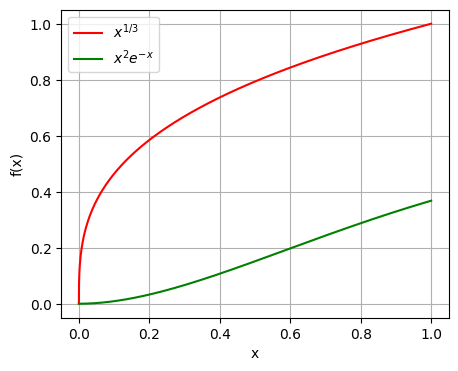
\includegraphics[width=\textwidth]{HW5/f_a and f_b.png}
        \caption{$f(x) = x^{1/3}$ and $f(x) = x^2e^{-x}$}
        \label{fig:image2}
    \end{minipage}
\end{figure}
\end{question}

\begin{question}{Q3 Approximate the integrals in Problem 2(a) and 2(b) using Gaussian Quadrature with
 n=2, 3, 4, and 5. Report the number of function evaluations and compare the results
 with those obtained using Romberg Integration in Problem-2. [3.5 points]}

\begin{table}[H]
\centering
\begin{tabular}{c c c c c c}
\hline
$n$ & $GQ_n(x^{1/3})$ & $GQ_n(x^2 e^{-x})$ & \# function evaluations & $e_n(x^{1/3})$ & $e_n(x^2 e^{-x})$ \\
\hline
2 & 0.759778 & 0.159410 & 2 & 0.009778 & 0.001193 \\
3 & 0.753855 & 0.160595 & 3 & 0.003855 & 0.000008 \\
4 & 0.751946 & 0.160603 & 4 & 0.001946 & 0.000000 \\
5 & 0.751132 & 0.160603 & 5 & 0.001132 & 0.000000 \\
\hline
\end{tabular}
\caption{Gaussian Quadrature for , corresponding function evaluations, and error estimates.}
\label{tab:gq_with_error}
\end{table}

\begin{tcolorbox}
    Since the number of function evaluations is 2,3,4 and 5 for Gaussian Quadrature, we will these values to Romberg's $n$ = 0, 1 and 2 (corresponding to 2, 3 and 5 function evaluations respectively.)
\end{tcolorbox}

\begin{table}[H]
\centering
\begin{tabular}{c c c c c c}
\hline
$n$ & $R_{n,n}(x^{1/3})$ & $R_{n,n}(x^2e^{-x})$ & \# function evaluations & $\epsilon_{n,n}(x^{1/3})$ & $\epsilon_{n,n}(x^2e^{-x})$ \\
\hline
0 & 0.500000 & 0.183940 & 2 & 0.250000 & 0.023337 \\
1 & 0.695800 & 0.162402 & 3 & 0.054200 & 0.001799 \\
2 & 0.730634 & 0.160611 & 5 & 0.019366 & 0.000008 \\
\hline
\end{tabular}
\caption{Table with $n$, $R_{n,n}$, function evaluations, and absolute errors.}
\label{tab:rn_table}
\end{table}

\begin{table}[H]
\centering
\begin{tabular}{c | c c | c c}
\hline
\#F.E & $\epsilon_{n,n}(x^{1/3})$ (R) & $\epsilon_n(x^{1/3})$ (GQ) & $\epsilon_{n,n}(x^2e^{-x})$ (R) & $\epsilon_n(x^2 e^{-x})$ (GQ) \\
\hline
2 & 0.250000 & \textbf{\underline{0.009778}$_L$} & 0.023337 & \textbf{\underline{0.001193}$_L$} \\
3 & 0.054200 & \textbf{\underline{0.003855}$_L$} & 0.001799 & \textbf{\underline{0.000008}$_L$} \\
5 & 0.019366 & \textbf{\underline{0.001132}$_L$} & 0.000008 & \textbf{\underline{0.000000}$_L$} \\
\hline
\end{tabular}
\caption{Comparison of error values for function evaluations 2, 3, and 5, with errors from the Gaussian Quadrature (GQ) and Romberg (R) methods. The lesser error is marked in underline bold with subscript $_L$.}
\label{tab:comparison_error_func_evals}
\end{table}


\begin{tcolorbox}
    From Table \ref{tab:comparison_error_func_evals} it is evident that {\textbf{for the same number of function evaluations, Gaussian Quadrature gives lesser error than Romberg integration}} for both the problems.\\ \\ Also to be noted that for problem a), \textbf{to beat the gaussian quadrature corresponding to \underline{5 function evaluations}, Romberg requires n = 6 ($\epsilon_{6,6} = 0.000465$) that corresponds to \underline{65 evaluations}! }
\end{tcolorbox}

\end{question}
    
\end{document}



